\documentclass{article}
%\usepackage{arxiv}
\usepackage[utf8]{inputenc}
\usepackage[T1]{fontenc}
\usepackage{geometry}
\geometry{margin=1in}
\usepackage{amsmath,amssymb}
\usepackage{graphicx}
\usepackage{booktabs}
\usepackage{algorithm}
\usepackage{algorithmic}
\usepackage{float}
\usepackage{url}
\usepackage{hyperref}
\usepackage{cleveref}
\usepackage{microtype}
\usepackage{tikz}
\newenvironment{keywords}{\noindent\textbf{Keywords: }}{}
\usetikzlibrary{shapes.geometric,arrows.meta,positioning}
\title{Fast IAPWS-IF97 Evaluation: Profiling-Guided Loop Tiling and Shared-Power Scaling}

\author{Maohua Cheng \\
  School of Energy and Environment, Southeast University \\
  Nanjing 210096, China \\
  \texttt{cmh@seu.edu.cn}}

\date{}

\begin{document}

\maketitle

\begin{abstract}
The IAPWS-IF97 formulation is the international standard for water and steam thermodynamic properties,
but direct formula evaluation without optimization cannot meet the performance demands of compute-intensive applications 
requiring millions of property calculations. Existing fast direct formula evaluations achieve only limited acceleration 
through repeated squaring. 
Alternative methods such as TTSE and SBTL avoid direct evaluation but sacrifice formula-level accuracy. 
This paper presents two acceleration techniques that directly optimize the IAPWS-IF97 formula evaluation while 
maintaining full formula accuracy:
   profiling-guided loop tiling and shared-power scaling.
   Profiling-guided loop tiling partitions polynomial summation into cache-friendly tiles with empirically determined boundaries, 
   enabling more effective SIMD vectorization.
   Shared-power scaling exploits the mathematical relationship 
   between Gibbs/Helmholtz free energy polynomials and their partial derivatives to compute them simultaneously in a single pass, 
   eliminating redundant power calculations. A Rust-based software package, SEUIF97, implements these methods. 
   Benchmark results demonstrate 5x to 36x speedups over baseline implementations and 
   3.7x to 6.6x speedups over CoolProp IF97, the most widely used open-source implementation, with the largest improvements in Regions 1, 2, and 3.
\end{abstract}

\begin{keywords}
IAPWS-IF97; Thermodynamic properties; Polynomial evaluation; Loop tiling; Shared-power scaling; Performance optimization
\end{keywords}

\section{Introduction}

The IAPWS-IF97 formulation \cite{IAPWS-IF97} is the international standard for calculating thermodynamic properties of water and steam.
Since its release, it has become the de facto standard in power engineering, process simulation, and thermal system analysis \cite{Wagner2008}. Compute-intensive applications such as real-time simulation, system optimization, and digital twins require millions of property calculations per second, where evaluating Gibbs and Helmholtz free energy polynomials and their partial derivatives becomes a performance bottleneck. Achieving fast property calculations requires designing efficient evaluation methods for these integer-exponent polynomials.

Existing approaches to improving IAPWS-IF97 computational speed fall into two categories. The first category directly evaluates 
the IF97 formulas with limited optimization. 
Among open-source implementations, freesteam \cite{FreeSteam} and CoolProp IF97 \cite{CoolProp,CoolPropIF97} 
have applied the repeated squaring method in their C/C++ implementations to optimize integer power computation. 
Most other implementations, including widely used libraries, directly evaluate the formulas term by term 
without exploiting the polynomial structure for acceleration. 
The second category uses alternative formulations that avoid direct polynomial evaluation. IAPWS has proposed the TTSE (Tabular Taylor Series Expansion) \cite{TTSE} and SBTL (Spline-Based Table Lookup) \cite{SBTL} methods, which use precomputed tables with interpolation to achieve fast lookups. These methods are designed for extremely high-speed applications but sacrifice formula-level accuracy and require extensive precomputation and storage.

Despite these efforts, significant opportunities remain unexplored in direct formula evaluation: the optimal tile 
boundaries for IF97 polynomial evaluation have not been determined, limiting the effectiveness of compiler loop optimizations, 
and the scaling relationship between derivative-related power terms has not been exploited to eliminate redundant calculations.

This paper proposes two acceleration techniques that directly optimize the IAPWS-IF97 formula evaluation:
\begin{enumerate}
    \item \textbf{Profiling-guided loop tiling}: Partitioning polynomial summation into cache-friendly tiles with empirically determined boundaries, enabling more effective SIMD vectorization and loop unrolling
    \item \textbf{Shared-power scaling}: Exploiting the mathematical relationship between polynomials and their derivatives to compute shared power terms once and obtain derivative results by exponent scaling, eliminating redundant calculations
\end{enumerate}

The paper is organized as follows: Section 2 reviews the IAPWS-IF97 formulation; Section 3 details the acceleration techniques; Section 4 presents benchmark results; Section 5 describes the software implementation; and Section 6 concludes.

\section{IAPWS-IF97 Formulation Overview}

The IAPWS-IF97 formulation \cite{IAPWS-IF97} divides the thermodynamic phase diagram of water and steam into five regions, as shown in Figure \ref{fig:if97_regions}. The 2012 consolidated release (R7-97(2012)) is the current standard, supplemented by backward equations for multiple input parameter pairs across all regions.

\begin{figure}[H]
\centering
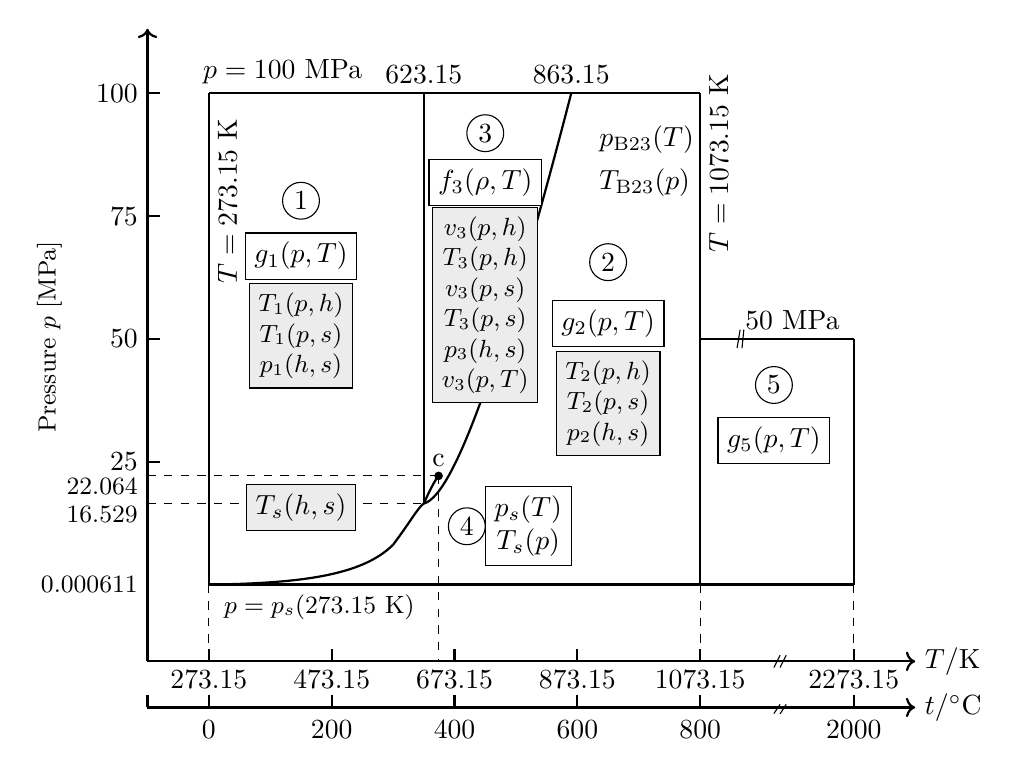
\begin{tikzpicture}[scale=0.78]
    % Axes
   
    % X-axis labels (T/K)
    \node[below] at (1.0,0) {273.15};
    \node[below] at (3.0,0) {473.15};
    \node[below] at (5.0,0) {673.15};
    \node[below] at (7.0,0) {873.15};
    \node[below] at (9.0,0) {1073.15};
    \node[below] at (11.5,0) {2273.15};
     % X-axis arrow and Temperature label
    \draw[->, thick] (0,0) -- (12.5,0);
    \node[right] at (12.5,0) {$T$/K};
     % x-axis tick vertical line
    \draw[black,thick] (1.0, 0) -- (1.0, 0.2);  
    \draw[black,thick] (3.0, 0) -- (3.0, 0.2);  
    \draw[black,thick] (5.0, 0) -- (5.0, 0.2);  
    \draw[black,thick] (7.0, 0) -- (7.0, 0.2);  
    \draw[black,thick] (9.0, 0) -- (9.0, 0.2);  
    \draw[black,thick] (11.5, 0) -- (11.5, 0.2);  
   
    % X-axis break
    \draw (10.2,-0.1) -- (10.3,0.1);
    \draw (10.3,-0.1) -- (10.4,0.1);
      
    % X-axis  second labels (t/°C)
    \node[below] at (1,-0.8) {0};
    \node[below] at (3.0,-0.8) {200};
    \node[below] at (5.0,-0.8) {400};
    \node[below] at (7.0,-0.8) {600};
    \node[below] at (9.0,-0.8) {800};
    \node[below] at (11.5,-0.8) {2000};
    % X-axis second row
    \draw[->, thick] (0,-0.75) -- (12.5,-0.75);
    \node[right] at (12.5,-0.75) {$t/^\circ$C};

     % x-axis tick vertical line
    \draw[black,thick] (0, -0.75) -- (0, -0.55);  
    \draw[black,thick] (1.0, -0.75) -- (1.0, -0.55);  
    \draw[black,thick] (3.0, -0.75) -- (3.0, -0.55);  
    \draw[black,thick] (5.0, -0.75) -- (5.0, -0.55);  
    \draw[black,thick] (7.0, -0.75) -- (7.0, -0.55);  
    \draw[black,thick] (9.0, -0.75) -- (9.0, -0.55);  
    \draw[black,thick] (11.5, -0.75) -- (11.5, -0.55);

     % X-axis second break
    \draw (10.2,-0.85) -- (10.3,-0.70);
    \draw (10.3,-0.855) -- (10.4,-0.70);
      
    % Y-axis arrow
    \draw[->, thick] (0,0) -- (0,10.3);
     % Y-axis labels (p/MPa)
    \node[left, font=\small] at (0,1.25) {0.000611};
    \node[left, font=\small, yshift=-4pt] at (0,2.57) {16.529};
    \node[left, font=\small, yshift=-4pt] at (0,3.02) {22.064};
    \node[left] at (0,3.25) {25};
    \node[left] at (0,5.25) {50};
    \node[left] at (0,7.25) {75};
    \node[left] at (0,9.25) {100};
    
      % Y-axis label
    \node[rotate=90, left=0.7cm, font=\small] at (-0.7,7.0) {Pressure $p$ [MPa]};

    % Y-axis tick line
    \draw[black,thick] (0, 3.25) -- (0.2,3.25);  
    \draw[black,thick] (0,5.25) -- (0.2, 5.25);  
    \draw[black,thick] (0,7.25) -- (0.2, 7.25);  
    \draw[black,thick] (0,9.25) -- (0.2, 9.25);
    
    % Region boundaries - solid lines
    % Left boundary T = 273.15 K
    \draw[thick] (1,1.25) -- (1.0,9.25);
    \node[rotate=90, right] at (1.3,6.0) {$T = 273.15$ K};
    
    % Top boundary p = 100 MPa
    \draw[thick] (1.0,9.25) -- (9.0,9.25);
    \node[above] at (2.2,9.25) {$p = 100$ MPa};
    
    % Isobar p = 22.064 MPa (dashed line from Y-axis to T=647.096)
    \draw[dashed] (0,3.02) -- (4.74,3.02);
    
    % Isobar p = 16.529 MPa (dashed line from Y-axis to T=623.15)
    \draw[dashed] (0,2.57) -- (4.5,2.57);
    
    % Isotherm T = 647.096 K (dashed line from critical point to X-axis)
    \draw[dashed] (4.74,3.02) -- (4.74,0);
    
    % T = 623.15 K vertical line (starts from saturation curve at p=16.529)
    \draw[thick] (4.5,2.57) -- (4.5,9.25);
    \node[above] at (4.5,9.25) {$623.15$};

     % T = 863.15 K label
    \node[above] at (6.9,9.25) {$863.15$};
    
    % T = 1073.15 K vertical line
    \draw[thick] (9.0,1.25) -- (9.0,9.25);
    \node[rotate=90, right] at (9.3,6.5) {$T = 1073.15$ K};
    
    % Dashed line from T=1073.15 to X-axis
    \draw[dashed] (9.0,1.25) -- (9.0,0);
    
     % T = 2273.15 K vertical line
    \draw[thick] (11.5,1.25) -- (11.5,5.25);
    
    % Dashed line from T=2273.15 to X-axis
    \draw[dashed] (11.5,1.25) -- (11.5,0);
    
    % p = 50 MPa horizontal line (Region 5)
    \draw[thick] (9.0,5.25) -- (11.5,5.25);
    \node[above] at (10.5,5.25) {50 MPa};
     %  p = 50 MPa horizontal lines break
    \draw (9.6,5.1) -- (9.65,5.4);
    \draw (9.68,5.1) -- (9.71,5.4);
    
    % Bottom boundary p = p_s(273.15 K) ≈ 0.000611 MPa
    \draw[thick] (1.0,1.25) -- (11.5,1.25);
    \node[below, font=\small] at (2.8,1.25) {$p = p_s(273.15$ K)};
    
    % Dashed line from T=273.15 to X-axis
    \draw[dashed] (1.0,1.25) -- (1.0,0);
    
    % Saturation curve (Region 4) - from triple point through (T=623.15, p=16.529) to critical point (T=647.096, p=22.064)
    % Starts very flat, gradually curves upward, steeper near critical point
    \draw[thick] (1.0,1.25) .. controls (2.5,1.27) and (3.5,1.4) .. (4.0,1.9);
    \draw[thick] (4.0,1.9) .. controls (4.3,2.3) and (4.4,2.5) .. (4.5,2.57);
    \draw[thick] (4.5,2.57) .. controls (4.6,2.8) and (4.7,2.98) .. (4.74,3.02);
    
    % Critical point (p=22.064 MPa, T=647.096 K)
    \fill (4.74,3.02) circle (2pt);
    \node[above] at (4.74,3.02) {c};
    
    % p_B23(T) curve - starts from (T=623.15, p=16.529) on saturation curve, curves right-up to (T=863.15, p=100)
    % Initial segment bends right below saturation curve
    \draw[thick] (4.5,2.57) .. controls (5.0,2.7) and (5.8,5.0) .. (6.9,9.25);
    \node[right] at (7.2,8.5) {$p_{\text{B23}}(T)$};
    \node[right] at (7.2,7.8) {$T_{\text{B23}}(p)$};
    
    % Region 1 - left side
    \draw (2.5,7.5) circle (0.3);
    \node at (2.5,7.5) {1};
    \node[draw, fill=gray!00, align=center] at (2.5,6.6) {$g_1(p,T)$};
    \node[draw, fill=gray!15, align=center, font=\small] at (2.5,5.3) {$T_1(p,h)$\\$T_1(p,s)$\\$p_1(h,s)$};
    
    % Region 2 - right side (larger area, elements shifted right)
    \draw (7.5,6.5) circle (0.3);
    \node at (7.5,6.5) {2};
    \node[draw, fill=gray!00, align=center] at (7.5,5.5) {$g_2(p,T)$};
    \node[draw, fill=gray!15, align=center, font=\small] at (7.5,4.2) {$T_2(p,h)$\\$T_2(p,s)$\\$p_2(h,s)$};
    
    % Region 3 - top middle (narrow strip between T=623.15K and p_B23 curve)
    \draw (5.5,8.6) circle (0.3);
    \node at (5.5,8.6) {3};
    \node[draw, fill=gray!00, align=center] at (5.5,7.8) {$f_3(\rho,T)$};
    \node[draw, fill=gray!15, align=center, font=\small] at (5.5,5.8) {$v_3(p,h)$\\$T_3(p,h)$\\$v_3(p,s)$\\$T_3(p,s)$\\$p_3(h,s)$\\$v_3(p,T)$};
    
    % Region 4 - saturation curve area
    \draw (5.2,2.2) circle (0.3);
    \node at (5.2,2.2) {4};
    \node[draw, fill=gray!00, align=center] at (6.2,2.2) {$p_s(T)$\\$T_s(p)$};
    \node[draw, fill=gray!15, align=center] at (2.5,2.5) {$T_s(h,s)$};
    
    % Region 5 - far right
    % T = 2273.15 K vertical line
    \draw (10.2,4.5) circle (0.3);
    \node at (10.2,4.5) {5};
    \node[draw, fill=gray!00, align=center] at (10.2,3.6) {$g_5(p,T)$};
    
\end{tikzpicture}
\caption{Structure and regions of IAPWS-IF97}
\label{fig:if97_regions}
\end{figure}

In addition, IAPWS \cite{IAPWS-Releases} provides formulations for transport properties, interfacial properties, and dielectric properties.

\subsection{Basic Equations}

The core of IAPWS-IF97 consists of two types of fundamental equations  for specific thermodynamic regions (Regions 1, 2, 3, and 5). Region 4 (saturation line) provides explicit equations for saturation pressure $p_s(T)$ and saturation temperature $T_s(p)$.

\subsubsection{Gibbs Free Energy Equation (Regions 1, 2, 5)}

Regions 1 (compressed liquid), 2 (superheated vapor), and 5 (high-temperature steam) use the dimensionless Gibbs free energy $g/(RT)$ as the fundamental equation. For Regions 2 and 5, the dimensionless Gibbs free energy is split into an ideal-gas part $\gamma^0$ and a residual part $\gamma^r$:

\begin{equation}
\frac{g(p,T)}{RT} = \gamma(\pi,\tau) = \gamma^0(\pi,\tau) + \gamma^r(\pi,\tau)
\label{eq:gibbs}
\end{equation}

where the reduced variables are defined as $\pi = p/p^{*}$ and $\tau = T^{*}/T$, with region-specific scaling parameters $p^{*}$ and $T^{*}$. The ideal-gas part $\gamma^0$ has the form:

\begin{equation}
\gamma^0(\pi,\tau) = \ln\pi + \sum_{i=1}^{N_0} n_i^0 \, \tau^{J_i^0}
\label{eq:gibbs_ideal}
\end{equation}

The residual part $\gamma^r$ is a polynomial in $\pi$ and $\tau$:

\begin{equation}
\gamma^r(\pi,\tau) = \sum_{i=1}^{N_r} n_i \, \pi^{I_i} \, \tau^{J_i}
\label{eq:gibbs_residual}
\end{equation}

For Region 1, the fundamental equation uses a single polynomial with shifted variables:

\begin{equation}
\gamma(\pi,\tau) = \sum_{i=1}^{N} n_i \, (7.1 - \pi)^{I_i} \, (\tau - 1.222)^{J_i}
\label{eq:gibbs_r1}
\end{equation}

where $\pi = p/p^{*}$ with $p^{*} = 16.53$ MPa and $\tau = T^{*}/T$ with $T^{*} = 1386$ K. The coefficients $n_i$ and exponents $I_i$, $J_i$ are provided in tabular form for each region. Table \ref{tab:region_params} summarizes the scaling parameters for each region.

\begin{table}[H]
\centering
\caption{Scaling parameters for Regions 1, 2, and 5}
\label{tab:region_params}
\begin{tabular}{lccc}
\toprule
\textbf{Region} & \textbf{Equation} & \textbf{$p^{*}$ (MPa)} & \textbf{$T^{*}$ (K)} \\
\midrule
1 (Liquid) & Gibbs & 16.53 & 1386  \\
2 (Vapor) & Gibbs & 1.0 & 540  \\
5 (High-T) & Gibbs & 1.0 & 1000  \\
\bottomrule
\end{tabular}
\end{table}

\subsubsection{Helmholtz Free Energy Equation (Region 3)}

Region 3 (near-critical region) uses the dimensionless Helmholtz free energy $f/(RT)$ as the fundamental equation, with density $\rho$ and temperature $T$ as independent variables:

\begin{equation}
\frac{f(\rho,T)}{RT} = \phi(\delta,\tau) = n_1 \ln\delta + \sum_{i=1}^{N} n_i \, \delta^{I_i} \, \tau^{J_i}
\label{eq:helmholtz}
\end{equation}

where $\delta = \rho/\rho^{*}$ and $\tau = T^{*}/T$, with $\rho^{*} = 322$ kg/m$^3$ and $T^{*} = 647.096$ K. The leading $n_1 \ln\delta$ term captures the ideal-gas behavior, and the 39 polynomial terms model the residual contribution.

\subsubsection{Summary of Fundamental Equations}

Table \ref{tab:formula_char} summarizes the key characteristics of the fundamental equations. These directly influence the computational cost and motivate the acceleration techniques.

\begin{table}[H]
\centering
\caption{IAPWS-IF97 formula characteristics by region}
\label{tab:formula_char}
\begin{tabular}{lccl}
\toprule
\textbf{Region} & \textbf{Terms} & \textbf{Exponent Range} & \textbf{Formulation} \\
\midrule
1 (Liquid) & 34 & $I_i$: 0--32, $J_i$: $-41$--17 & Gibbs \\
2 (Vapor) & 9 + 43 & $I_i$: 1--24, $J_i$: $-5$--58 & Gibbs (ideal + residual) \\
3 (Critical) & 1 + 39 & $I_i$: 0--11, $J_i$: 0--26 & Helmholtz ($\ln\delta$ + polynomial) \\
4 (Saturation) & 10 & --- & Exponential \\
5 (High-T) & 6 + 6 & $I_i$: 1--3, $J_i$: $-3$--9 & Gibbs (ideal + residual) \\
\bottomrule
\end{tabular}
\end{table}

\subsection{Thermodynamic Property Derivation}
\label{sec:thermodynamic_property_derivation}

Thermodynamic properties are derived from the fundamental equations and their partial derivatives: Gibbs free energy $\gamma(\pi,\tau)$ in Regions 1, 2, and 5, and Helmholtz free energy $\phi(\delta,\tau)$ in Region 3. Taking Region 2 as a representative example, the key properties derived from $\gamma(\pi,\tau) = \gamma^0(\pi,\tau) + \gamma^r(\pi,\tau)$ are:

\begin{align}
h &= RT \cdot \tau \left( \gamma^0_\tau + \gamma^r_\tau \right) \label{eq:enthalpy} \\
s &= R \left[ \tau \left( \gamma^0_\tau + \gamma^r_\tau \right) - \left( \gamma^0 + \gamma^r \right) \right] \label{eq:entropy} \\
w^2 &= RT \cdot \frac{1 + 2\pi\gamma^r_\pi + \pi^2(\gamma^r_\pi)^2}{\left( 1 - \pi^2\gamma^r_{\pi\pi} \right) + \dfrac{\left( 1 + \pi\gamma^r_\pi - \tau\pi\gamma^r_{\pi\tau} \right)^2}{\tau^2\left( \gamma^0_{\tau\tau} + \gamma^r_{\tau\tau} \right)}} \label{eq:speed}
\end{align}

Other properties such as specific volume $v = \frac{RT}{p}(\gamma^0_\pi + \gamma^r_\pi)$ and specific isobaric heat capacity $c_p = -R\tau^2(\gamma^0_{\tau\tau} + \gamma^r_{\tau\tau})$ follow the same pattern.

A key observation is that the partial derivatives share the same power terms as the original equations, only with modified coefficients. Taking the residual part $\gamma^r$ and its partial derivative with respect to $\tau$ as an example:

\begin{equation}\label{eq:gibbs_residual_tau}
\left( \frac{\partial \gamma^r}{\partial \tau} \right)_\pi = \sum_{i=1}^{N_r} (n_i J_i) \, \pi^{I_i} \, \tau^{J_i - 1} =\frac{1}{\tau} \sum_{i=1}^{N_r} (n_i J_i) \, \pi^{I_i} \, \tau^{J_i}
\end{equation}

Comparing Eq.~(\ref{eq:gibbs_residual_tau}) with Eq.~(\ref{eq:gibbs_residual}), both share the identical base power product $\pi^{I_i} \tau^{J_i}$ and differ only in their coefficient multipliers ($n_i$ vs. $n_i J_i$). This shared structure enables the shared-power scaling technique described in Section \ref{sec:shared_power_scaling}.

\subsection{Backward Equations}

The backward equations are integer-power polynomials for inverse property calculations. For example, the backward equation $T(p,h)$ for subregion 2a reads:

\begin{equation}\label{eq:backward_eq_reg2_ph_t_2a}
\frac{T_{2a}(p,h)}{T^*} = \theta_{2a}(\pi,\eta) = \sum_{i=1}^{34} n_i \, \pi^{I_i} (\eta - 2.1)^{J_i}
\end{equation}

where $\theta = T/T^*$, $\pi = p/p^*$, and $\eta = h/h^*$ with $T^* = 1$ K, $p^* = 1$ MPa, and $h^* = 2000$ kJ kg$^{-1}$. The 34 coefficients $n_i$ and exponents $I_i$, $J_i$ are provided in tabular form in the IAPWS supplementary release. Similar backward equations exist for other input parameter pairs across all regions, benefiting from the same acceleration techniques as the fundamental equations. 

\subsection{Formula Characteristics}

Three key characteristics motivate the acceleration techniques:

\textbf{Characteristic 1: Integer exponents.} All fundamental and backward equations are sums of terms $n_i x^{I_i} y^{J_i}$ with integer $I_i$, $J_i$, enabling efficient integer power operations. In C/C++ implementations, this typically requires manual optimization such as repeated squaring, while Rust provides a built-in integer power function \texttt{powi()} that the compiler optimizes aggressively as an intrinsic.

\textbf{Characteristic 2: Shared power terms.} The partial derivatives share the same base power products with the original equations, differing only in coefficients. For example, when computing specific entropy $s$ in Region 2, both $\gamma^r$ and $\gamma^r_\tau$ share the identical base power product $\pi^{I_i}\tau^{J_i}$ (Section \ref{sec:thermodynamic_property_derivation}). This enables shared-power scaling.

\textbf{Characteristic 3: High term counts.} The fundamental and backward equations in the main regions contain numerous terms, 
making polynomial evaluation the dominant computational cost. For example, Regions 1 and 2 contain 34 and 52 terms respectively (Table \ref{tab:formula_char}). 
This enables loop tiling.

\section{Acceleration Techniques}

\subsection{Profiling-Guided Loop Tiling}

Loop tiling (also known as loop blocking) \cite{LoopTiling,Grosser2012Polly} is a general optimization technique that partitions a single loop into multiple smaller loops (tiles) to improve cache locality and enable effective SIMD vectorization. Modern compilers can automatically vectorize simple loops, but without appropriate tile boundaries, the compiler's optimization potential remains limited due to register pressure and cache constraints.

The critical challenge in applying loop tiling is determining the optimal tile boundaries for a specific computational problem. For IF97 polynomial evaluation, the boundaries depend on complex interactions between polynomial term count, CPU cache hierarchy, and compiler optimization behavior. This paper addresses this challenge through empirical performance profiling: for Region 2 (43 residual terms), profiling reveals that three tiles (0--13, 13--26, and 26--43) yield the best results, enabling more effective SIMD vectorization and loop unrolling. The optimal tile boundaries identified through profiling are hard-coded into the polynomial evaluation functions for each region and property type.

Algorithm \ref{alg:loop_tiling} presents the tiled polynomial evaluation:

\begin{algorithm}[H]
\caption{Loop Tiling for Single Polynomial (for $N$ terms partitioned into $M$ tiles)}
\label{alg:loop_tiling}
\begin{algorithmic}[1]
\REQUIRE $x, y$: reduced variables (e.g., $\pi, \tau$ for Regions 2/5; $7.1{-}\pi, \tau{-}1.222$ for Region 1; $\delta, \tau$ for Region 3)
\REQUIRE $IJn$: array of $(I_i, J_i, n_i)$ polynomial coefficients
\REQUIRE $\text{steps}$: array of $(start, end)$ tile boundaries
\ENSURE $S = \sum_i n_i x^{I_i} y^{J_i}$: polynomial summation result

\STATE Initialize $S \leftarrow 0$
\FOR{each tile $m$ in $\text{steps}$}
    \FOR{$k \leftarrow \text{steps}[m].start$ \TO $\text{steps}[m].end - 1$}
        \STATE $term \leftarrow IJn[k].n \times x^{IJn[k].I} \times y^{IJn[k].J}$
        \STATE $S \leftarrow S + term$
    \ENDFOR
\ENDFOR
\RETURN $S$
\end{algorithmic}
\end{algorithm}

Loop tiling provides the most significant speedup for polynomials with many terms (Regions 1, 2, and 3), as shown in Table~\ref{tab:benchmarks}. For polynomials with few terms (Region 5, 12 terms total), loop tiling is selectively applied based on profiling results.

\subsection{Shared-Power Scaling}
\label{sec:shared_power_scaling}

Shared-power scaling computes the base power product once per term and obtains derivatives by scaling with the corresponding exponents, eliminating redundant calculations.

For example, entropy $s$ in Region 2 (Eq.~\ref{eq:entropy}) requires both $\gamma$ and $\gamma_\tau$.  Since $\gamma^r$ and $\gamma^r_\tau$ share the base power product $\pi^{I_i}\tau^{J_i}$ (Eqs.~\eqref{eq:gibbs_residual} and \eqref{eq:gibbs_residual_tau}), each term is computed once and accumulated to both results simultaneously. The $\gamma^r_\tau$ accumulator collects $(n_i J_i) \pi^{I_i}\tau^{J_i}$ and is divided by $\tau$ after the loop.
The same principle applies to the ideal-gas part $\gamma^0$ and its derivative $\gamma^0_\tau$, which share the power terms $\tau^{J_i^0}$.

Algorithm \ref{alg:scaling} presents the shared-power scaling approach for derivative-related polynomial computation combined with loop tiling, for the case of computing the polynomial value and its two first-order partial derivatives simultaneously:

\begin{algorithm}[H]
\caption{Shared-Power Scaling with Loop Tiling}
\label{alg:scaling}
\begin{algorithmic}[1]
\REQUIRE $x, y$: reduced variables (e.g., $\pi, \tau$ for Regions 2/5; $7.1{-}\pi, \tau{-}1.222$ for Region 1; $\delta, \tau$ for Region 3)
\REQUIRE $IJn$: array of $(I_i, J_i, n_i)$ polynomial coefficients
\REQUIRE $\text{steps}$: array of $(start, end)$ tile boundaries
\ENSURE $\gamma, \partial\gamma/\partial x, \partial\gamma/\partial y$: polynomial and its partial derivatives

\STATE Initialize $\gamma \leftarrow 0$, $\gamma_x \leftarrow 0$, $\gamma_y \leftarrow 0$
\FOR{each tile $m$ in $\text{steps}$}
    \FOR{$k \leftarrow \text{steps}[m].start$ \TO $\text{steps}[m].end - 1$}
        \STATE $term \leftarrow IJn[k].n \times x^{IJn[k].I} \times y^{IJn[k].J}$
        \STATE $\gamma \leftarrow \gamma + term$
        \STATE $\gamma_x \leftarrow \gamma_x + IJn[k].I \times term$
        \STATE $\gamma_y \leftarrow \gamma_y + IJn[k].J \times term$
    \ENDFOR
\ENDFOR
\STATE $\gamma_x \leftarrow \gamma_x / x$
\STATE $\gamma_y \leftarrow \gamma_y / y$
\RETURN $(\gamma, \gamma_x, \gamma_y)$
\end{algorithmic}
\end{algorithm}

For properties requiring only one derivative (e.g., entropy $s$ needs $\gamma$ and $\gamma_\tau$), the same pattern applies with only the relevant derivative accumulator active. For properties requiring higher-order or mixed derivatives (e.g., speed of sound $w$), additional accumulators are added following the same coefficient-multiplication principle.

\subsection{Combined Application}

The two techniques are applied based on the computational requirements of each property:

\begin{itemize}
    \item \textbf{Profiling-guided loop tiling}: Applied to polynomial summations where profiling demonstrates performance improvement (typically Regions 1, 2, and 3 with many terms). For properties with few terms (Region 5), loop tiling is omitted as the tile overhead may outweigh the benefits.
    \item \textbf{Shared-power scaling}: Applied to all properties requiring both the polynomial and its derivatives, 
    such as entropy  $s$ (which requires $\gamma_\tau$,$\gamma$) and $w$ (which requires $\gamma_\pi$, $\gamma_{\pi\pi}$, $\gamma_{\pi\tau}$, $\gamma_{\tau\tau}$). The shared-power scaling technique computes all required derivatives simultaneously, eliminating redundant power calculations.
\end{itemize}

These techniques are orthogonal and can be applied independently. For example, Region 5 entropy $s$ computation uses shared-power scaling alone, while Region 2 enthalpy $h$ uses profiling-guided loop tiling alone (Table~\ref{tab:benchmarks}). When both techniques are applicable, they are combined for maximum performance improvement.

\section{Performance Benchmarks}
\label{sec:performance-benchmarks}

All benchmarks were conducted on the same hardware: an Intel Core i7-1165G7 @ 2.80~GHz processor with 8~GB DDR4 RAM. 
These benchmark was performed on Windows 11. SEUIF97 was compiled using Rust 1.96.0 in release mode with \texttt{opt-level = 3} and \texttt{target-cpu = native}.
Note that the two benchmarks use different measurement frameworks; therefore, absolute execution times are not directly comparable across tables.

\subsection{Speedup over Baseline Implementation}

The first benchmark evaluates the proposed acceleration techniques 
by comparing the optimized SEUIF97 implementation against a baseline 
that uses only Rust's built-in integer power function \texttt{powi()} with a single loop, without loop tiling or shared-power scaling. 
Both implementations evaluate the IF97 basic equations.
Measurements were conducted using the Criterion framework \cite{Criterion}.

Table~\ref{tab:benchmarks} shows the results for representative points in each region.
\begin{table}[H]
\centering
\small
\caption{Speedup over baseline (\texttt{powi()} with single loop)}
\label{tab:benchmarks}
\begin{tabular}{@{}lcllccc@{}}
\toprule
\textbf{Case} & \textbf{Reg.} & \textbf{Input} & \textbf{Method} & \textbf{Baseline (ns)} & \textbf{Acc. (ns)} & \textbf{Speedup} \\
\midrule
$(p,T)\!\rightarrow\!h$ & 1 & 3.0 MPa, 300 K & Loop tiling & 767.3 & 37.0 & 20.7x \\
$(p,T)\!\rightarrow\!s$ & 1 & 3.0 MPa, 300 K & Loop tiling + Shared-power scaling & 1449.9 & 41.5 & 34.9x \\
$(p,T)\!\rightarrow\!h$ & 2 & 0.0035 MPa, 300 K & Loop tiling & 1042.2 & 45.9 & 23.7x \\
$(p,T)\!\rightarrow\!s$ & 2 & 0.0035 MPa, 300 K & Loop tiling + Shared-power scaling & 2076.3 & 57.8 & 35.9x \\
$(T,v)\!\rightarrow\!h$ & 3 & 650 K, 0.002 m$^3$/kg & Loop tiling & 1835.8 & 120.8 & 15.2x \\
$(T,v)\!\rightarrow\!s$ & 3 & 650 K, 0.002 m$^3$/kg & Loop tiling + Shared-power scaling & 1968.8 & 116.2 & 16.9x \\
$(p,T)\!\rightarrow\!h$ & 5 & 0.5 MPa, 1500 K & Baseline & 9.7 & --- & --- \\
$(p,T)\!\rightarrow\!s$ & 5 & 0.5 MPa, 1500 K & Shared-power scaling & 75.1 & 14.8 & 5.1x \\
\bottomrule
\end{tabular}
\end{table}

The results show significant speedups across all regions, with the largest improvements in Regions 1, 2, and 3 where the polynomial forms are most complex. Region 5, with only 12 terms (6 ideal + 6 residual), has relatively low computational cost, so the optimization techniques provide limited benefit.

\subsection{Comparison with CoolProp IF97}

The second benchmark compares SEUIF97 against CoolProp IF97 \cite{CoolPropIF97}, the most widely used open-source C++ implementation of IF97 on GitHub. CoolProp IF97 employs its own optimized repeated-squaring fast integer power algorithm, making it representative of existing optimized implementations.
CoolProp IF97 was compiled using MSVC 19.50.35719.0 with \texttt{-O3} and \texttt{-march=native} optimization. Measurements were performed using \texttt{clock\_t} \cite{MusserClock2024}.

Table~\ref{tab:benchmarks_seuif97_coolprop_if97} shows the comparison results.
Note that Region 3 results use backward equations $(p,T)$ since CoolProp IF97 does not implement the $(T,v)$ fundamental equation interface.

\begin{table}[H]
\centering
\small
\caption{SEUIF97 vs. CoolProp IF97}
\label{tab:benchmarks_seuif97_coolprop_if97}
\begin{tabular}{@{}lclccc@{}}
\toprule
\textbf{Case} & \textbf{Reg.} & \textbf{Input} & \textbf{CoolProp IF97 (ns)} & \textbf{SEUIF97 (ns)} & \textbf{Speedup} \\
\midrule
$(p,T)\!\rightarrow\!h$ & 1 & 3.0 MPa, 300 K & 151.1 & 41.4 & 3.7x \\
$(p,T)\!\rightarrow\!s$ & 1 & 3.0 MPa, 300 K & 246.3 & 46.1 & 5.3x \\
$(p,T)\!\rightarrow\!h$ & 2 & 0.0035 MPa, 300 K & 207.9 & 47.4 & 4.4x \\
$(p,T)\!\rightarrow\!s$ & 2 & 0.0035 MPa, 300 K & 377.4 & 57.0 & 6.6x \\
$(p,T)\!\rightarrow\!h$ & 3 & 50 MPa, 630 K & 389.5 & 89.3 & 4.4x \\
$(p,T)\!\rightarrow\!s$ & 3 & 50 MPa, 630 K & 422.1 & 83.1 & 5.1x \\
$(p,T)\!\rightarrow\!h$ & 5 & 0.5 MPa, 1500 K & 54.2 & 9.9 & 5.5x \\
$(p,T)\!\rightarrow\!s$ & 5 & 0.5 MPa, 1500 K & 74.8 & 16.8 & 4.5x \\
\bottomrule
\end{tabular}
\end{table}

SEUIF97 achieves 3.7--6.6x speedups over CoolProp IF97. These gains stem from the proposed algorithmic optimizations.

\section{Software Implementation: SEUIF97}
\label{sec:software-implementation-seuif97}  
SEUIF97 is a Rust-based IAPWS-IF97 property calculation library following a modular three-layer architecture:

\begin{enumerate}
    \item \textbf{Public API}: User-facing functions supporting multiple input parameter pairs (p-T, p-h, p-s, etc.)
    \item \textbf{Region wrapper}: Region-specific functions handling coordinate transformations and step boundary definitions
    \item \textbf{Optimized kernel}: A family of tile-based polynomial evaluation functions implementing loop tiling and shared-power scaling
\end{enumerate}

This layered design ensures flexibility while maintaining optimal performance. The architecture is illustrated in Figure \ref{fig:architecture}.

\begin{figure}[H]
\centering
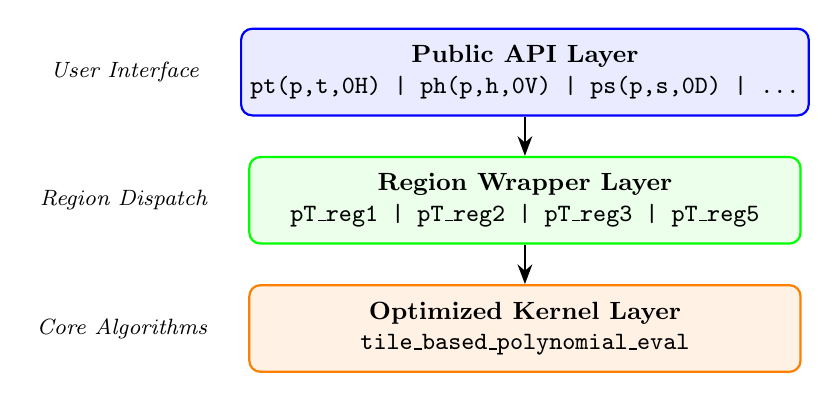
\begin{tikzpicture}[
    box/.style={rectangle, rounded corners, draw, thick, minimum width=7cm, minimum height=1.1cm, align=center, font=\small},
    arrow/.style={-{Stealth[length=2.5mm]}, thick},
    label/.style={font=\footnotesize\itshape, align=right}
]
    \node[box, fill=blue!8, draw=blue] (api) {
        \textbf{Public API Layer}\\
        \texttt{pt(p,t,0H) | ph(p,h,0V) | ps(p,s,0D) | \ldots}
    };
    \node[label, left=0.4cm of api] (l1) {User Interface};

    \node[box, fill=green!8, draw=green, below=0.5cm of api] (wrapper) {
        \textbf{Region Wrapper Layer}\\
        \texttt{pT\_reg1 | pT\_reg2 | pT\_reg3 | pT\_reg5}
    };
    \node[label, left=0.4cm of wrapper] (l2) {Region Dispatch};

    \node[box, fill=orange!10, draw=orange, below=0.5cm of wrapper] (kernel) {
        \textbf{Optimized Kernel Layer}\\
        \texttt{tile\_based\_polynomial\_eval}
    };
    \node[label, left=0.4cm of kernel] (l3) {Core Algorithms};

    \draw[arrow] (api.south) -- (wrapper.north);
    \draw[arrow] (wrapper.south) -- (kernel.north);
\end{tikzpicture}
\caption{Three-layer architecture of SEUIF97}
\label{fig:architecture}
\end{figure}

SEUIF97 supports 12 input parameter pairs ($(p,t)$, $(p,h)$, $(p,s)$, $(p,v)$, $(t,h)$, $(t,s)$, $(t,v)$, $(h,s)$, $(p,x)$, $(t,x)$, $(h,x)$, $(s,x)$, where $x$ is vapor quality) and computes 36 thermodynamic, transport, and derived properties.

SEUIF97 is available as a Rust crate on crates.io, a Python package on PyPI, a WebAssembly module on npm, and  shared library with C bindings. The source code is at \texttt{https://github.com/thermalogic/RustSEUIF97} under the MIT license.

\section{Conclusions}

This paper proposes two acceleration techniques for the IAPWS-IF97 formula evaluation: profiling-guided loop tiling and
shared-power scaling in derivative-related polynomials. The key insight is that the IAPWS-IF97 fundamental equations and their partial derivatives share the same power terms, 
enabling simultaneous computation in a single pass. Combined with profiling-guided loop tiling for cache optimization, 
the proposed approach achieves 5x to 36x speedups over baseline implementations that use fast integer power functions with a single loop (Table~\ref{tab:benchmarks}), and 14x to 30x speedups over CoolProp IF97 (Table~\ref{tab:benchmarks_seuif97_coolprop_if97}), with the largest improvements in Regions 1, 2, and 3 where the polynomial forms are most complex. 
These results demonstrate that direct IAPWS-IF97 formula evaluation can achieve substantial speedup while maintaining full formula accuracy, substantially improving performance for compute-intensive applications. SEUIF97 is available as a Rust crate, Python package, WebAssembly module, and shared library with C bindings.



\begin{thebibliography}{99}

\bibitem{IAPWS-IF97}
IAPWS, ``R7-97(2012): Revised Release on the IAPWS Industrial Formulation 1997 for the Thermodynamic Properties of Water and Steam,'' International Association for the Properties of Water and Steam, 2012.

\bibitem{Wagner2008}
W. Wagner, H.-J. Kretzschmar, ``International Steam Tables: Properties of Water and Steam Based on the Industrial Formulation IAPWS-IF97,'' 2nd ed., Springer, Berlin, 2008.

\bibitem{FreeSteam}
John Pye, ``freesteam: Open source steam property routines in C,'' SourceForge. [Online]. Available: \url{https://sourceforge.net/projects/freesteam/}. Accessed: Jun. 6, 2026.

\bibitem{CoolProp}
I.H. Bell, J. Wronski, S. Quoilin, and V. Lemort, ``Pure and Pseudo-pure Fluid Thermophysical Property Evaluation and the Open-Source Thermophysical Property Library CoolProp,'' \textit{Industrial \& Engineering Chemistry Research}, vol. 53, no. 6, pp. 2498--2508, 2014.

\bibitem{CoolPropIF97}
Ian Bell and the CoolProp Team, ``CoolProp IF97: Open-source C++ implementation of the IAPWS-IF97 equations,'' GitHub, 2023. [Online]. Available: \url{https://github.com/CoolProp/IF97}. Accessed: Jun. 6, 2026.

\bibitem{TTSE}
IAPWS, ``Release on the Tabular Taylor Series Expansion (TTSE) Method for the Calculation of Thermodynamic Properties of Water and Steam,'' International Association for the Properties of Water and Steam, 1997.

\bibitem{SBTL}
IAPWS, ``Release on the Spline-Based Table Lookup (SBTL) Method for the Calculation of Thermodynamic Properties of Water and Steam,'' International Association for the Properties of Water and Steam, 2015.

\bibitem{IAPWS-Releases}
IAPWS, ``IAPWS Releases, Supplementary Releases, Guidelines, and Advisory Notes,'' International Association for the Properties of Water and Steam, [Online]. Available: \url{https://iapws.org/documents/release}. Accessed: Jun. 6, 2026.

\bibitem{LoopTiling}
M.E. Wolf, M.S. Lam, ``A data locality optimizing algorithm,'' Proceedings of the ACM SIGPLAN Conference on Programming Language Design and Implementation, 1991, pp. 30-44.

\bibitem{Grosser2012Polly}
T. Grosser, A. Groesslinger and C. Lengauer, ``Polly - Performing polyhedral optimizations on a low-level intermediate representation,'' Parallel Process. Lett., vol. 22, no. 4, Dec. 2012.

\bibitem{Criterion}
Brook Heisler, ``Criterion.rs: Statistics-driven benchmarking library for Rust,'' GitHub, 2022. [Online]. Available: \url{https://github.com/bheisler/criterion.rs}. Accessed: Jun. 6, 2026.

\bibitem{MusserClock2024}
David R. Musser, ``Measuring Computing Times and Operation Counts,'' Rensselaer Polytechnic Institute (RPI), Oct 2024.
[Online]. Available: \url{https://cs.rpi.edu/~musser/gp/timing.html}. Accessed: Jun. 6, 2026.
\end{thebibliography}

\end{document}